% Created 2026-04-21 Tue 19:38
% Intended LaTeX compiler: lualatex
\DocumentMetadata{lang = en, pdfversion = 2.0, pdfstandard = ua-2, pdfstandard = a-4, testphase = {phase-III, title, table, math, firstaid}}
\documentclass[11pt]{article}
\usepackage{amsmath}
\usepackage{fontspec}
\usepackage{graphicx}
\usepackage{longtable}
\usepackage{wrapfig}
\usepackage{rotating}
\usepackage[normalem]{ulem}
\usepackage{capt-of}
\usepackage{hyperref}
\usepackage[margin=1in]{geometry}
\usepackage{fontspec}
\usepackage{verbatim, multicol, tabularx,}
\usepackage{amsmath, amsthm, amssymb, stmaryrd, latexsym, bm, listings, qtree}
\usepackage{framed}
\usepackage{xcolor,colortbl}
\usepackage{media9}
\usepackage[export]{adjustbox}
\usepackage{algorithm}
\usepackage[noend]{algpseudocode}
\usepackage{tikz,pgfplots}
\usetikzlibrary{shapes.geometric}
\let\oldquote=\quote
\let\endoldquote=\endquote
\colorlet{shadecolor}{cyan!15}
\renewenvironment{quote}{\begin{shaded*}\begin{oldquote}}{\end{oldquote}\end{shaded*}}
% From https://tex.stackexchange.com/questions/7032/good-way-to-make-textcircled-numbers
\newcommand*\circled[1]{\tikz[baseline=(char.base)]{\node[shape=circle,draw,inner sep=2pt] (char) {#1};}}
\DeclareMathOperator*{\argmin}{arg\!min}
\DeclareMathOperator*{\argmax}{arg\!max}
\lstset{frame=tb, aboveskip=1mm, belowskip=0mm, showstringspaces=false, columns=flexible, basicstyle={\scriptsize\ttfamily}, numbers=left, frame=single, breaklines=true, breakatwhitespace=true}
\hypersetup{colorlinks=true,urlcolor=blue}
\usepackage{polyglossia}
\setdefaultlanguage[variant=US]{english}
\author{Christopher Simpkins}
\date{Kennesaw State University}
\title{Artificial Intelligence\\\medskip
\large First-Order Logic}
\hypersetup{
 pdfauthor={Christopher Simpkins},
 pdftitle={Artificial Intelligence},
 pdfkeywords={},
 pdfsubject={Artificial Intelligence First-Order Logic},
 pdfcreator={Emacs 30.2 (Org mode 9.7.11)}, 
 pdflang={English}}
\begin{document}

\maketitle
\section{Representation}
\label{sec:orgcecb5e0}


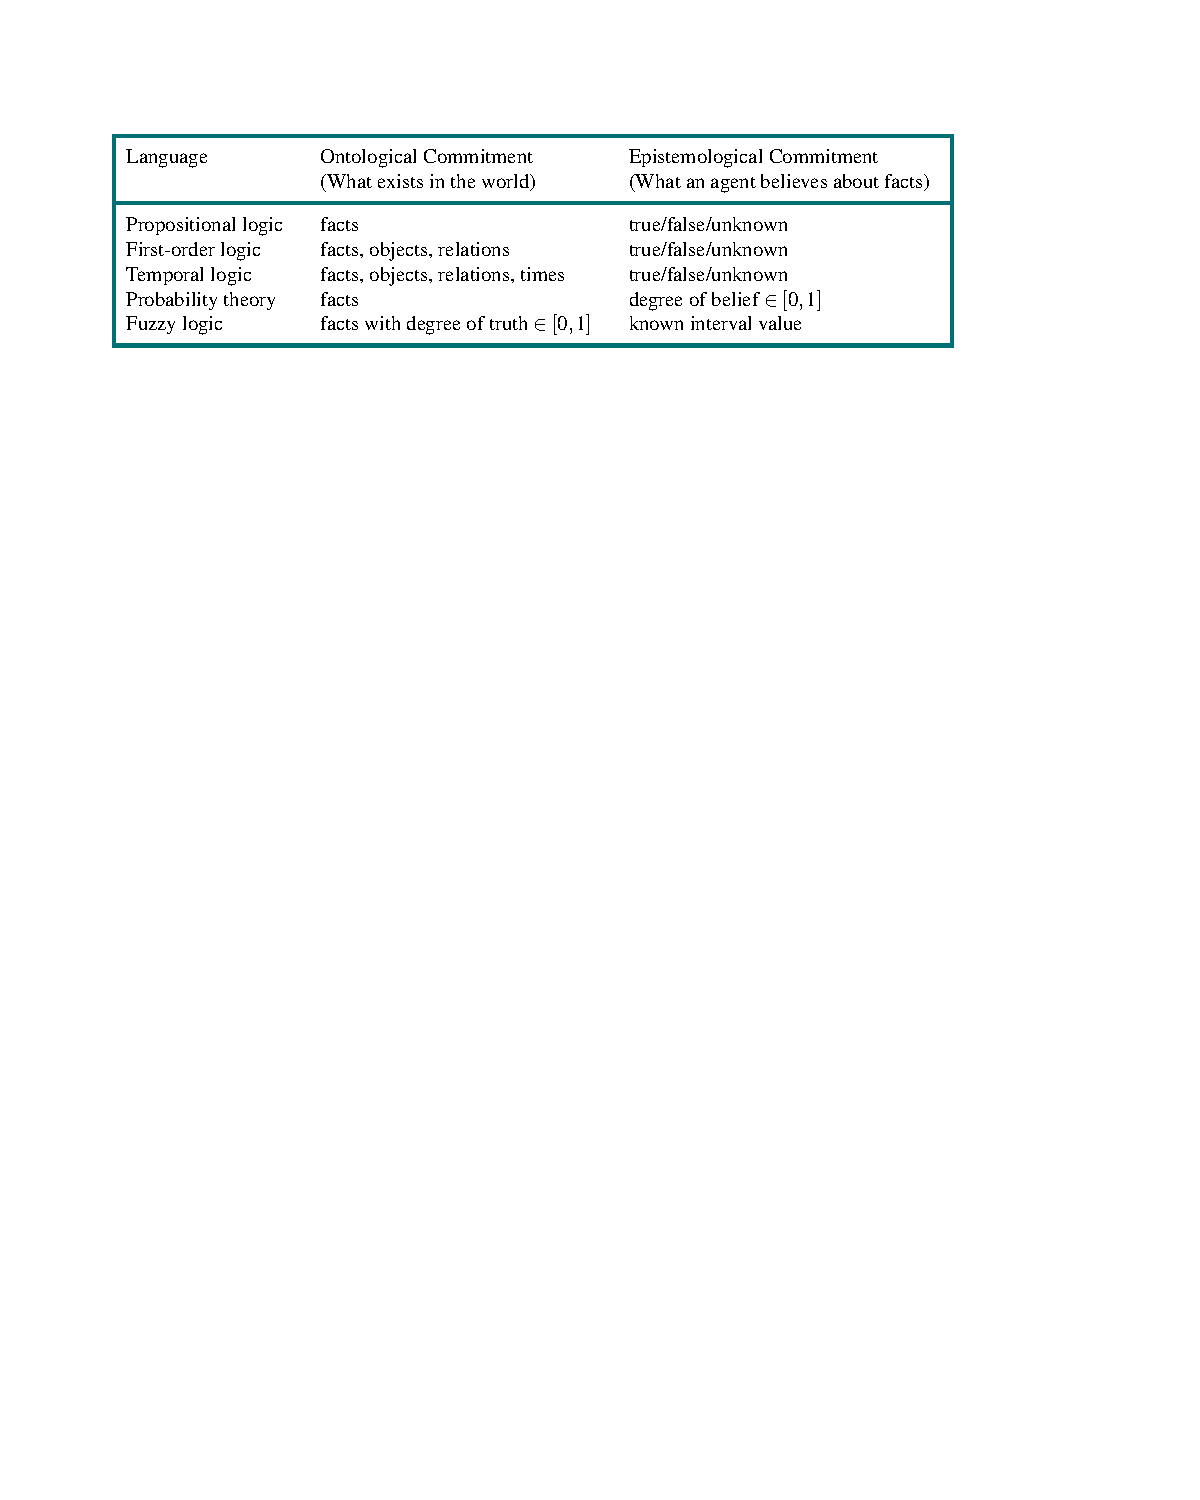
\includegraphics[alt={aima fig 08_01 ontological epistemological commitments},height=1in]{aima-fig-08_01-ontological-epistemological-commitments.pdf}
\section{Syntax and Semantics of First-Order Logic}
\label{sec:org17e4cb4}


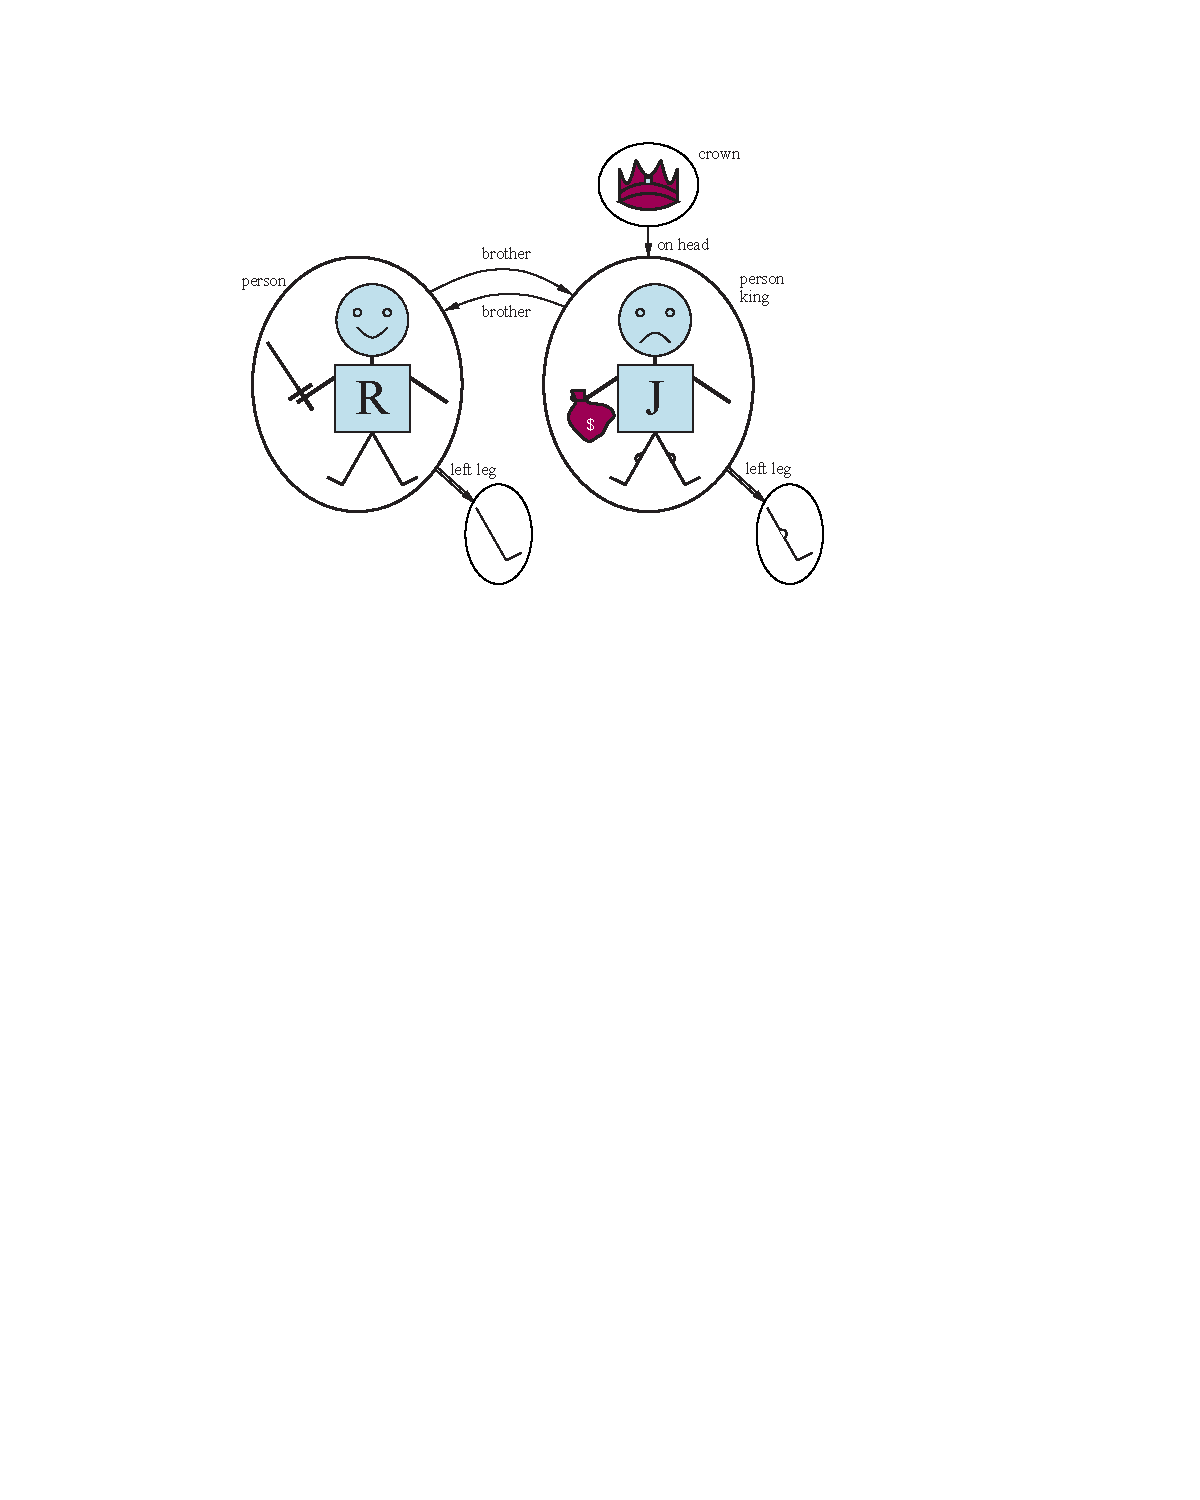
\includegraphics[alt={aima fig 08_02 person king model},height=1in]{aima-fig-08_02-person-king-model.pdf}
\section{Syntax and Semantics of First-Order Logic}
\label{sec:org6bbb2df}


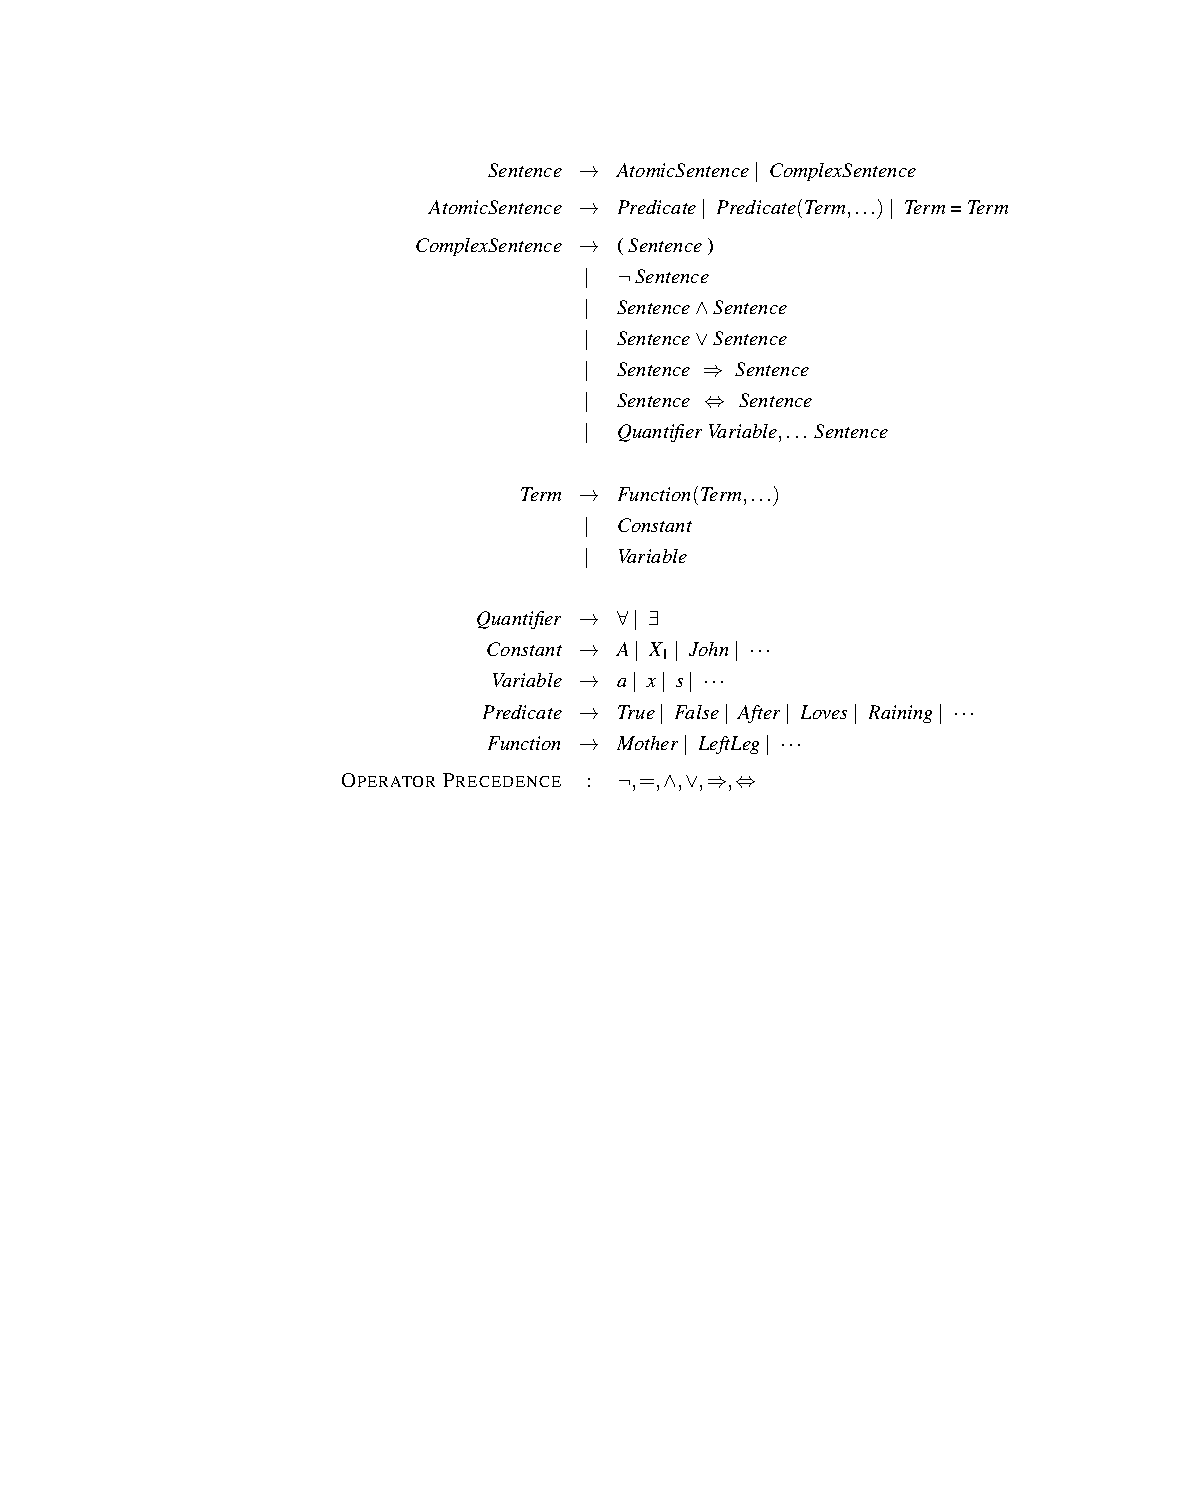
\includegraphics[alt={aima fig 08_03 syntax of fol},height=1in]{aima-fig-08_03-syntax-of-fol.pdf}
\section{Syntax and Semantics of First-Order Logic}
\label{sec:org9b90f8e}


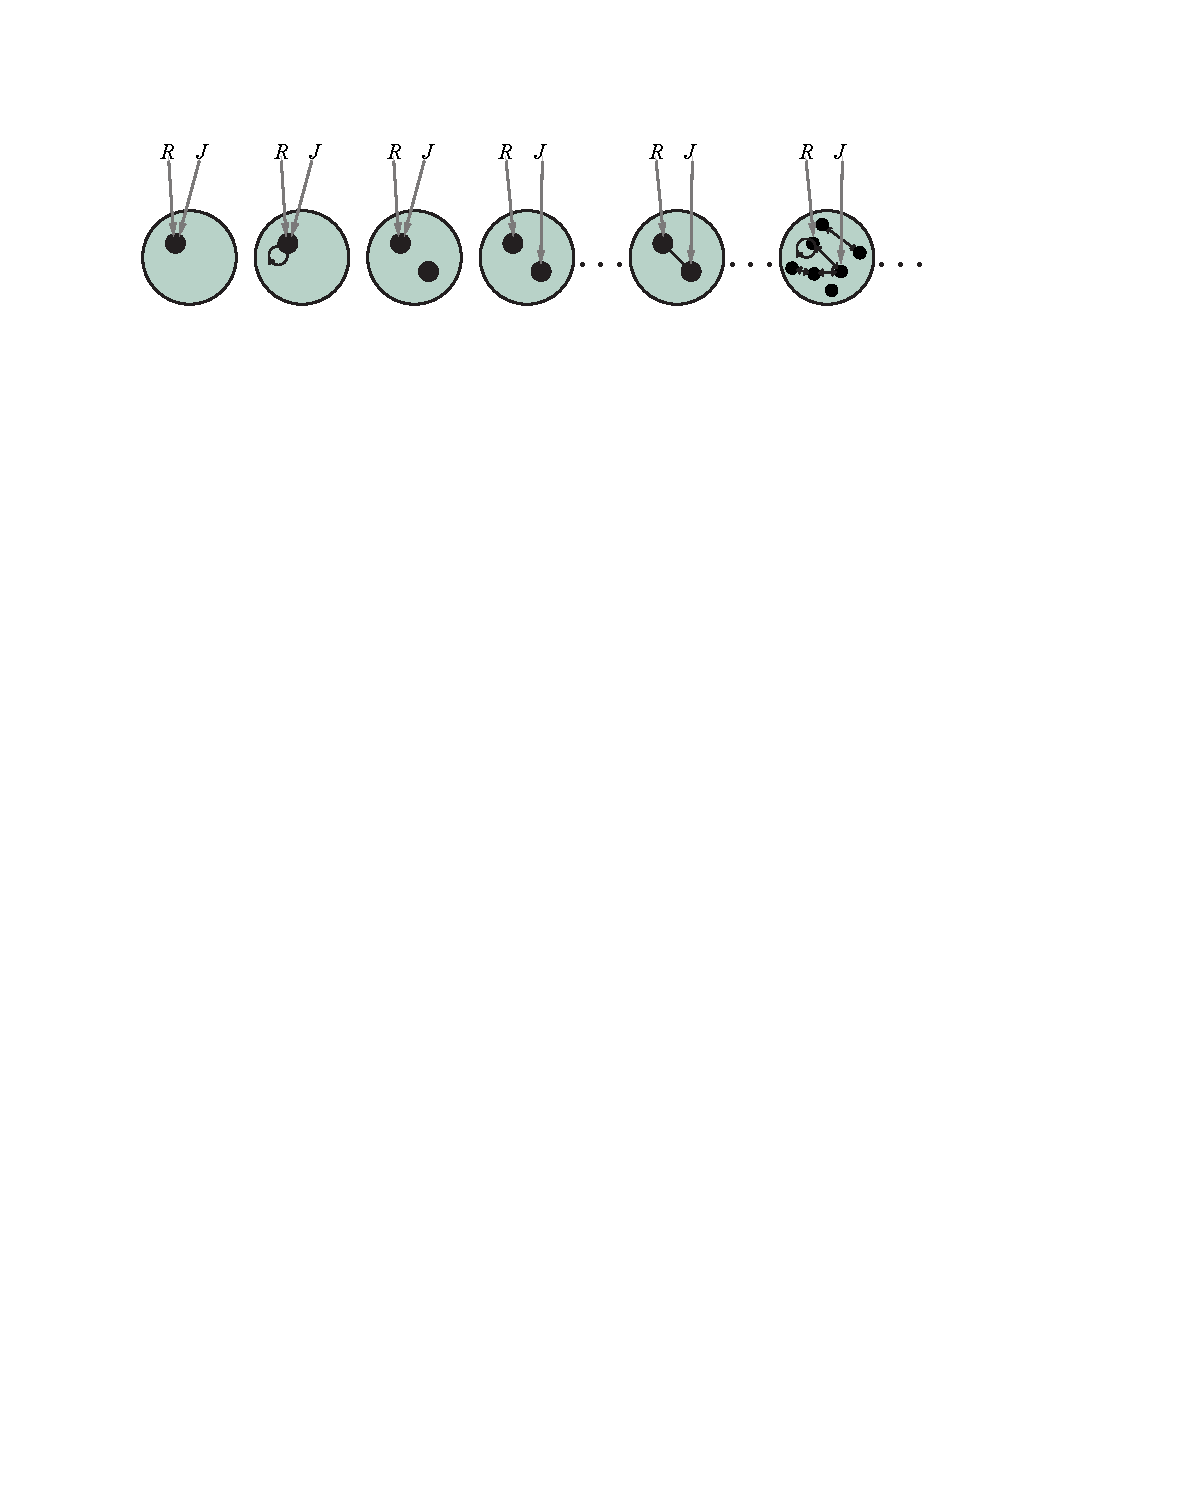
\includegraphics[alt={aima fig 08_04 simple example models},height=1in]{aima-fig-08_04-simple-example-models.pdf}
\section{Syntax and Semantics of First-Order Logic}
\label{sec:org007d903}


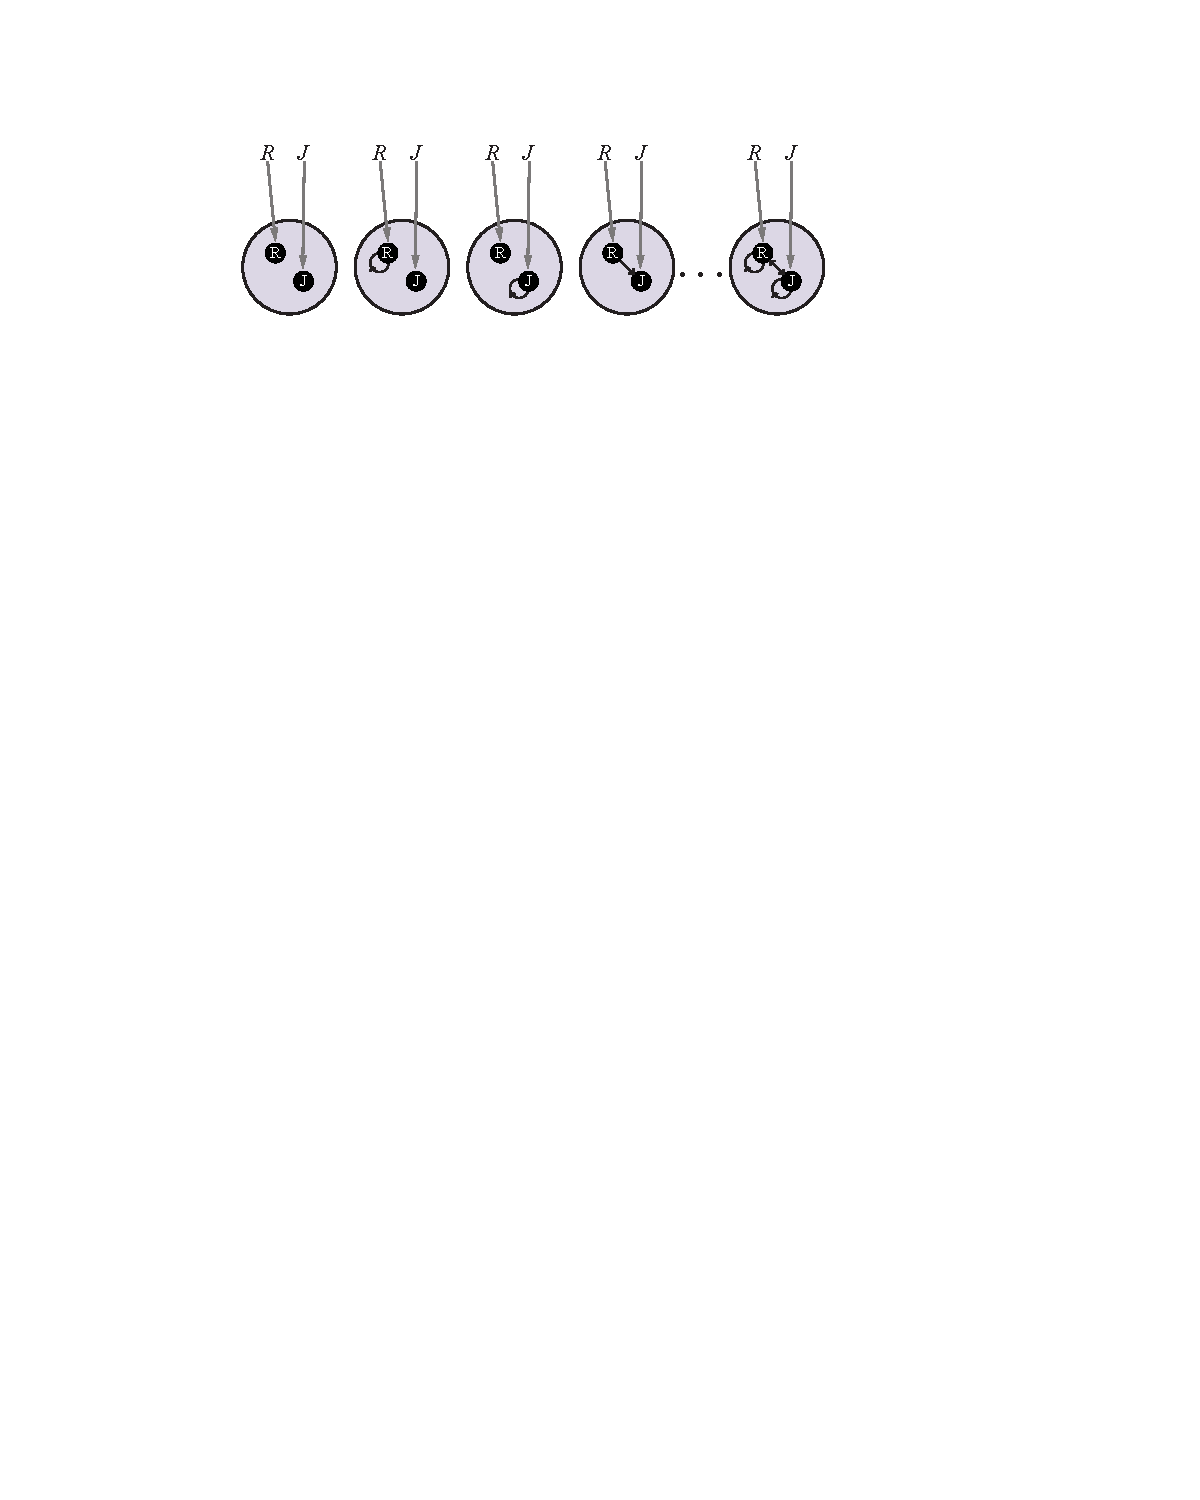
\includegraphics[alt={aima fig 08_05 simple example models database semantics},height=1in]{aima-fig-08_05-simple-example-models-database-semantics.pdf}
\section{Using First-Order Logic}
\label{sec:orgd11c0d6}

Foo
\section{Knowledge Engineering in First-Order Logic}
\label{sec:org77992f8}


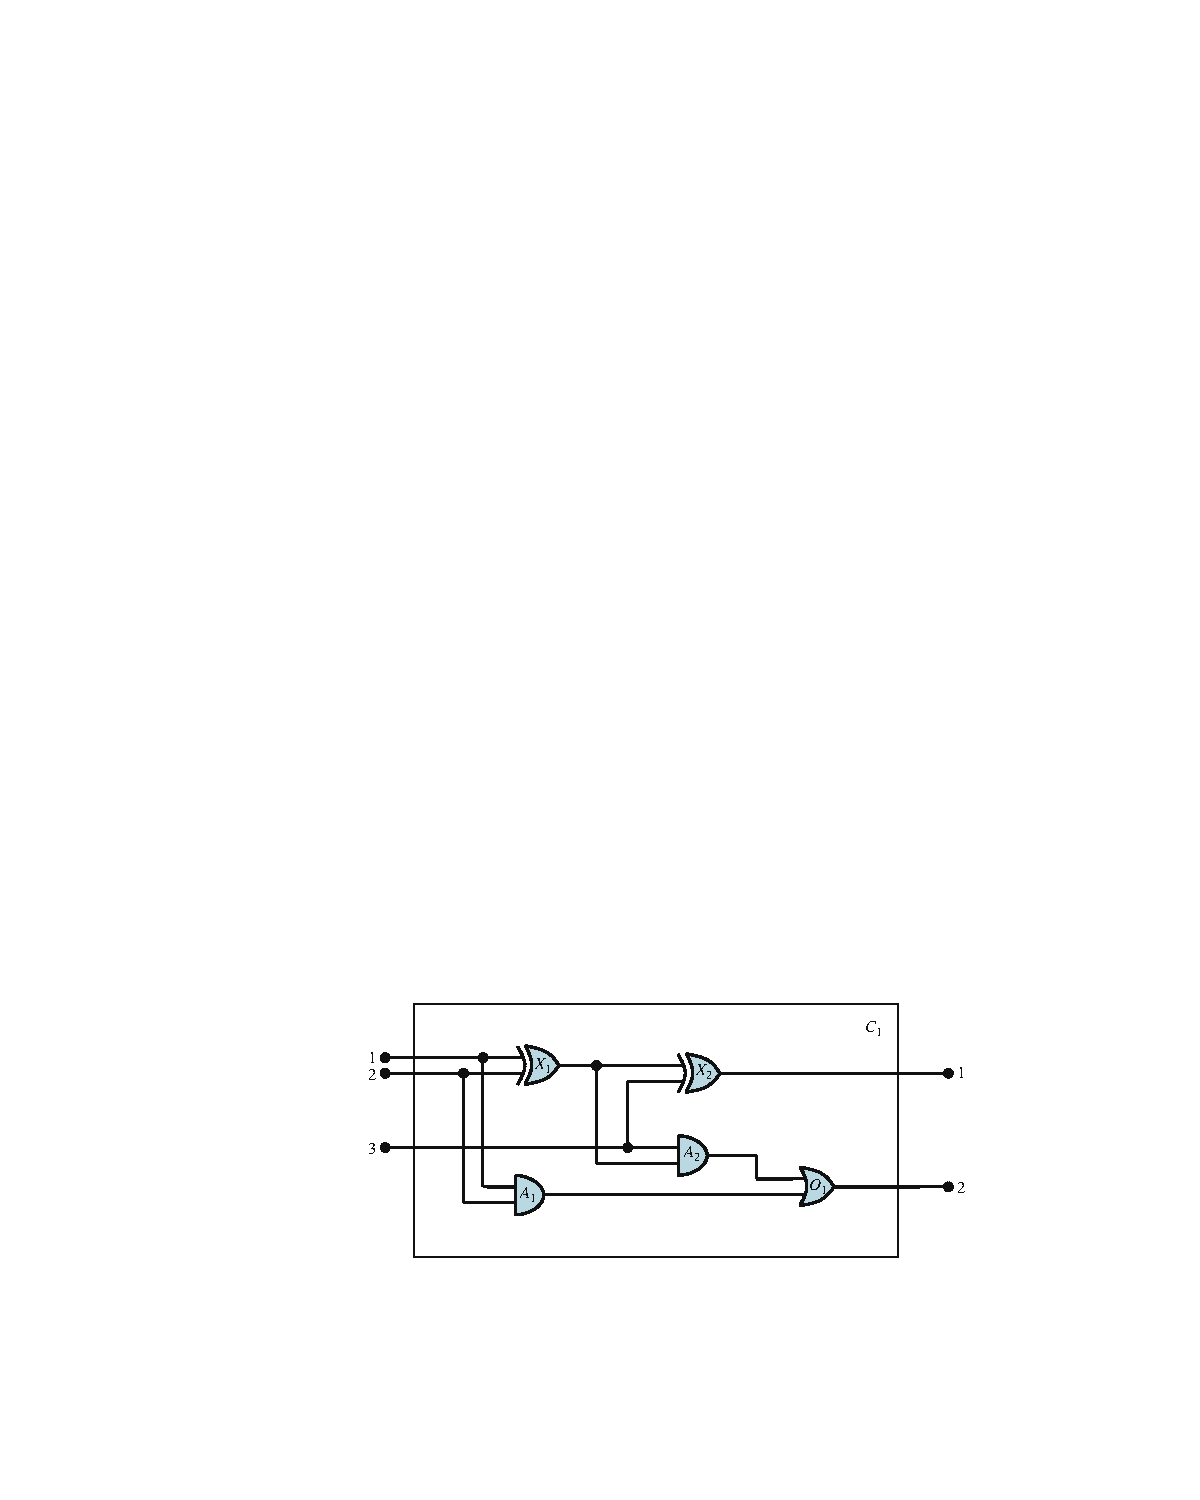
\includegraphics[alt={aima fig 08_06 digital circuit},height=1in]{aima-fig-08_06-digital-circuit.pdf}
\end{document}
